\documentclass{paper}

%\usepackage{times}
\usepackage{epsfig}
\usepackage{graphicx}
\usepackage{amsmath}
\usepackage{amssymb}
\usepackage{color}
\usepackage{caption}
\usepackage{subcaption}


% load package with ``framed'' and ``numbered'' option.
%\usepackage[framed,numbered,autolinebreaks,useliterate]{mcode}

% something NOT relevant to the usage of the package.
\setlength{\parindent}{0pt}
\setlength{\parskip}{18pt}






\usepackage[latin1]{inputenc} 
\usepackage[T1]{fontenc} 

\usepackage{listings} 
\lstset{% 
   language=Matlab, 
   basicstyle=\small\ttfamily, 
} 



\title{Assignment 1}



\author{Simon Jenni\\09-116-005}
% //////////////////////////////////////////////////


\begin{document}



\maketitle


% Add figures:
%\begin{figure}[t]
%%\begin{center}
%\quad\quad   \includegraphics[width=1\linewidth]{ass2}
%%\end{center}
%
%\label{fig:performance}
%\end{figure}

\section*{Superresolution}

\begin{enumerate}
\item \textbf{Problem.} The goal of superresolution is to recover high resolution images of given low resolution input images. This problem can be modelled mathematically by assuming the following image creation model: 
\begin{equation}\label{eq:contProblem}
g(x,y)=(u*k)(\alpha x, \alpha y).
\end{equation}
Here, $g$ is the low resolution input image that results from down-sampling a higher resolution image $u$ with an averaging filter $k$ and down-sampling factor $\alpha$. The task of superresolution therefore is to find $u$ given $g$, $k$ and $\alpha$.

As we deal with images in the discrete, equation \ref{eq:contProblem} can be rewritten as
\begin{equation}
g=Du.
\end{equation}
In this case, $g$ and $u$ are column vectors (column-major ordering of the images) and $D$ is a down-sampling matrix. The solution $u$ can now be found by minimising 
\begin{equation}\label{eq:energy}
E(u)=\frac{\lambda}{2}||Du-g||^2+||\nabla u||
\end{equation}
with respect to $u$.  Here, $||\nabla u||$ is equal to a Total Variation (TV) regularisation term which ensures a certain smoothness in the output image $u$ and the parameter $\lambda$ controls the trade-off between minimising the error and regularisation terms. The image we are looking for is therefore given by
\begin{equation}\label{eq:solution}
\tilde{u}=\arg\min_{u} E(u)
\end{equation}

\item \textbf{Motivations.} There are many applications of superresolution we can think of. Any situation where the highest possible resolution of a screen is higher than the resolution of some image is a possible use-case. While being more computationally expensive than a simple interpolation scheme, superresolution results in a higher perceived quality of the up-scaled images and allows humans to better interpret these. Superresolution could also be used to save space while storing or transmitting images. Concrete use-cases are mobile-phone images used as wallpaper, the enlargement of a sub window of an image, retrieval of mug shots from surveillance cameras, and so on.

\item \textbf{Derivation of gradient.} To numerically solve for the best image $u$ in equation \ref{eq:solution}, the energy given by equation \ref{eq:energy} is discretised. Using forward finite differences for the approximation leads to:
\begin{equation}\label{eq:objDisc}
E(u)=\frac{\lambda}{2}\sum_{i,j}((Du)(i,j)-g(i,j))^2+\sum_{i,j}\tau (i,j)
\end{equation}
where 
\begin{equation}\label{eq:tau}
\tau (i,j)=\sqrt{(u(i+1,j)-u(i,j))^2+(u(i,j+1)-u(i,j))^2}.
\end{equation}
To minimise equation \ref{eq:objDisc} we use a gradient-descent approach with the update rule 
\begin{equation}\label{eq:GD}
u:=u-\alpha\nabla_{u}E. 
\end{equation}

This of course requires the computation of the gradient $\nabla_{u}E$ of equation \ref{eq:objDisc} with respect to $u$:
\begin{equation}\label{eq:gradientE}
\nabla_{u}E=\lambda D^T(Du-g)+\frac{\partial}{\partial u}||\nabla u||
\end{equation}
where the entries of $\frac{\partial}{\partial u}||\nabla u||$ in turn are computed by
\begin{equation}\label{eq:gradTau}
\frac{\partial ||\nabla u||}{\partial u(i,j)}=\frac{\partial \tau (i,j)}{\partial u(i,j)}+\frac{\partial \tau (i-1,j)}{\partial u(i,j)}+\frac{\partial \tau (i,j-1)}{\partial u(i,j)}
\end{equation}
with the partial derivatives of $\tau$ w.r.t u given by:
\begin{equation}\label{eq:gradTau1}
\frac{\partial \tau (i,j)}{\partial u(i,j)}=\frac{2u(i,j)-u(i+1,j)-u(i,j+1)}{\tau(i,j)}
\end{equation}
\begin{equation}\label{eq:gradTau2}
\frac{\partial \tau (i-1,j)}{\partial u(i,j)}=\frac{u(i,j)-u(i-1,j)}{\tau(i-1,j)}
\end{equation}
\begin{equation}\label{eq:gradTau3}
\frac{\partial \tau (i,j-1)}{\partial u(i,j)}=\frac{u(i,j)-u(i,j-1)}{\tau(i,j-1)}
\end{equation}



\item \textbf{Implement gradient descent for superresolution.} 
I implemented a gradient descent algorithm to solve for $u$. The computation of the gradient requires to make some boundary assumptions for $u$. The assumptions made here are that $u$ is mirrored along its boundaries. The updating-factor $\alpha$ in equation \ref{eq:GD} is determined via backtracking line search. Figure \ref{fig:iterations} shows results at different stages of the minimisation.
\begin{figure}[]
\begin{center}
	\begin{subfigure}[b]{0.49\textwidth}
                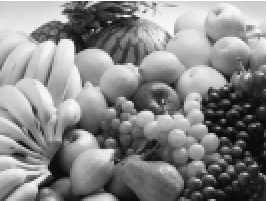
\includegraphics[width=\textwidth]{it1}
                \caption{1st Iteration}
        \end{subfigure}
        	\begin{subfigure}[b]{0.49\textwidth}
                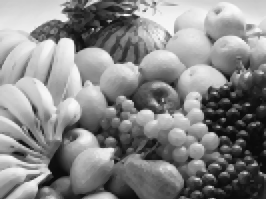
\includegraphics[width=\textwidth]{it600}
                \caption{600th Iteration}
        \end{subfigure}
        \begin{subfigure}[b]{0.49\textwidth}
                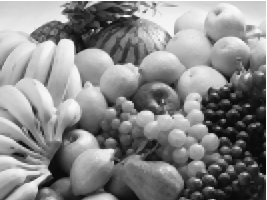
\includegraphics[width=\textwidth]{it1200}
                \caption{1200th Iteration}
        \end{subfigure}
        \begin{subfigure}[b]{0.49\textwidth}
                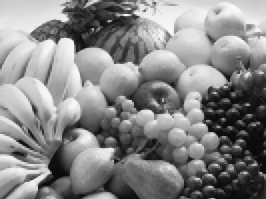
\includegraphics[width=\textwidth]{it1800}
                \caption{1800th Iteration}
        \end{subfigure}
        \begin{subfigure}[b]{0.49\textwidth}
                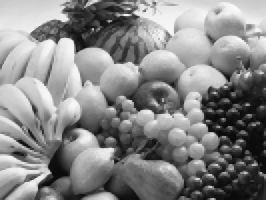
\includegraphics[width=\textwidth]{it2400}
                \caption{2400th Iteration}
        \end{subfigure}
        \begin{subfigure}[b]{0.49\textwidth}
                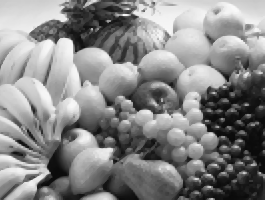
\includegraphics[width=\textwidth]{itfinal}
                \caption{Final Iteration (3000th)}
        \end{subfigure}
\end{center}
\caption{This figure shows an image at several different stages of the gradient descent algorithm. }
\label{fig:iterations}
\end{figure}

\item \textbf{The influence of $\lambda$.} 
The parameter $\lambda$ in equation \ref{eq:energy} controls the trade-off between minimising the error and minimising the regularisation term $||\nabla u||$. Figure \ref{fig:lambda} shows results for different values of $\lambda$. Setting it low places more weight on minimising $||\nabla u||$, therefore making $u$ smoother. Setting $\lambda$ high on the other hand places more weight on minimising the error between the low-res input image and the down-sampled prediction $u$, therefore $u$ will be more similar to an up-scaled version of the low-res input image (it will look more pixelated).
\begin{figure}[]
\begin{center}
	\begin{subfigure}[b]{0.49\textwidth}
                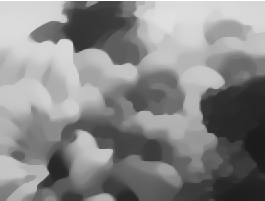
\includegraphics[width=\textwidth]{lambda10}
                \caption{$\lambda=10$ (low)}
        \end{subfigure}
        	\begin{subfigure}[b]{0.49\textwidth}
                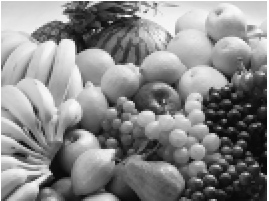
\includegraphics[width=\textwidth]{lambda1000000}
                \caption{$\lambda=1'000'000$ (high)}
        \end{subfigure}
        \begin{subfigure}[b]{0.49\textwidth}
                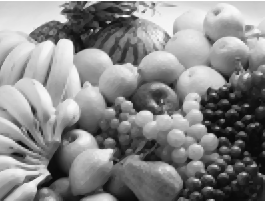
\includegraphics[width=\textwidth]{lambdaOpt}
                \caption{$\lambda=10'000$ (reasonable)}
        \end{subfigure}
\end{center}
\caption{This figure shows results for different values of the parameter $\lambda$. }
\label{fig:lambda}
\end{figure}

\item \textbf{ Find optimal $\lambda$.}

As we know the optimal value for $u$, we can look for the value of $\lambda$ which minimises the sum of squared distances (SSD) 
\begin{equation}
SSD(u)=\sum_{i,j}(\tilde{u}(i,j)-u(i,j))
\end{equation}
between the ground truth $u$ and the solution $\tilde{u}$ we computed. Figure \ref{fig:SSD} shows the SSD vs. $\lambda$ graph. We observe that very low values for $\lambda$ result in a very high SSD. For $\lambda$ between 5'000 and 40'000, the SSD stays nearly constant and increases again for $\lambda > 40'000$. The graph draws a convex function with a minimum at approximately $\lambda=33'500$.

\begin{figure}[]
\begin{center}
         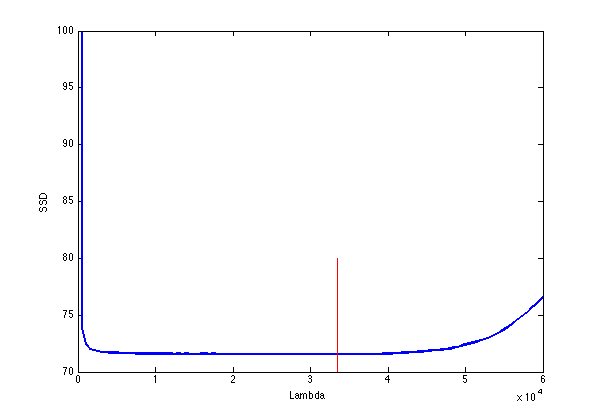
\includegraphics[width=\textwidth]{SSD}       
\end{center}
\caption{This figure shows the effect of $\lambda$ on the SSD between the ground-truth $u$ and our solution $\tilde{u}$. The red vertical line indicates the optimal value for $\lambda$.  }
\label{fig:SSD}
\end{figure}

\end{enumerate}


 \end{document}
 
 